\begin{figure}[ht]
  \begin{framed}
  	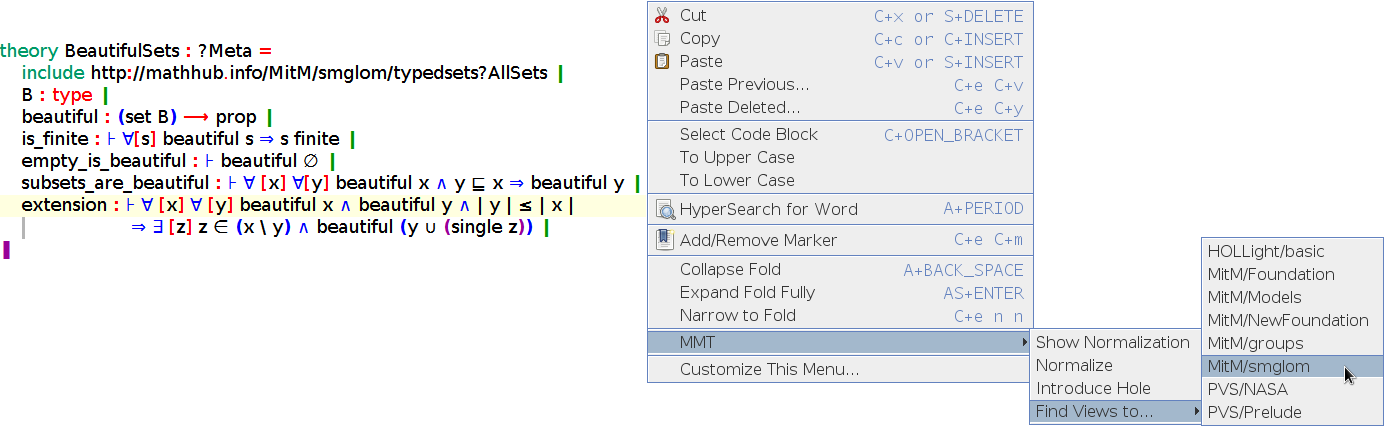
\includegraphics[width=\textwidth]{img/vf-beautysource}
  \end{framed}
  \caption{``Beautiful Sets'' in MMT Surface Syntax}\label{fig:use:source}
\end{figure}

I have implemented our view finder algorithm in the \mmt system and exposed it in \mmt's jEdit IDE.
A screenshot of Jane's theory of beautiful sets is given in \autoref{fig:use:source}.
Right-clicking anywhere within the theory allows Jane to select \cn{MMT} $\to$ \cn{Find} \cn{Views\ to...} $\to$ \cn{MitM/smglom}.
The latter menu offers a choice of known libraries in which the view finder should look for codomain theories; \cn{MitM/smglom} is the Math-in-the-Middle library (see \autoref{sec:lf:mitm}).

\noindent After choosing \cn{MitM/smglom}, the view finder finds two views (within less than one second) and shows them (\autoref{fig:use:results}).

\begin{figure}[ht]%r{.61\textwidth}\vspace*{-2em}
	\centering
  \fbox{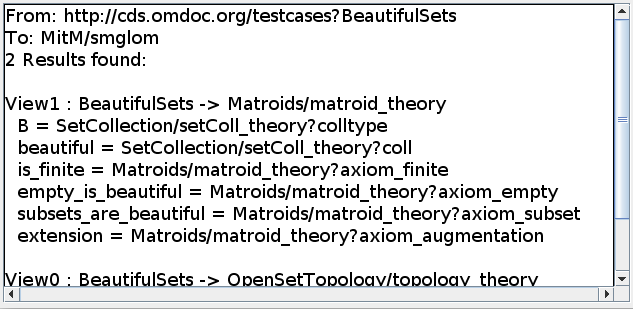
\includegraphics[width=0.6\textwidth]{img/vf-results}}  
  \caption{Views Found for ``Beautiful Sets''}\label{fig:use:results}%\vspace*{-2em}
\end{figure}

The first of these ($\cn{View1}$) has a theory for matroids as its codomain, which is given in \autoref{fig:use:target}.
Inspecting that theory and the assignments in the view, we see that it indeed represents the well-known correspondence between beautiful sets and matroids.

\begin{mmtcode}[caption={The Theory of Matroids in the MitM Library\protect\footnotemark},label=fig:use:target]
theory Matroids : base:?Logic =
	include ?Properties ❙
	include typedsets?FiniteCardinality ❙
	include arithmetics?NaturalArithmetics ❙

	theory matroid_theory : base:?Logic > X : type ❘ =
		include typedsets?SetCollection/setColl_theory (X) ❙
		
		axiom_finite : {s : set X} ⊦ s ∈ coll ⟶ ⊦ s finite ❙
		axiom_empty : ⊦ prop_emptyInColl coll ❙
		axiom_subset : ⊦ prop_subsetClosed coll ❙
		axiom_augmentation : ⊦ ∀ [A] ∀ [B] A ∈ coll ∧ B ∈ coll ∧ | B | ≤ | A | 
				⇒ ∃ [x] x ∈ (A \ B) ∧ (B ∪ (single x)) ∈ coll ❙
	❚
❚
\end{mmtcode}
\footnotetext{\url{https://gl.mathhub.info/MitM/smglom/blob/master/source/collections/matroids.mmt}}

%\begin{figure}[ht]%l{.61\textwidth}\vspace*{-2em}
%	\centering
%  \fbox{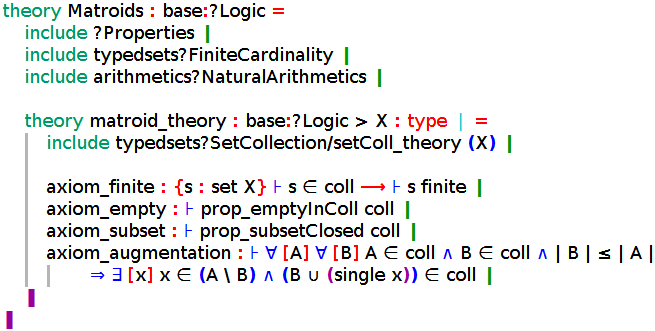
\includegraphics[width=0.6\textwidth]{img/vf-matroids}}%\vspace*{-.5em}
%  \caption{The Theory of Matroids in the MitM Library}\label{fig:use:target}%\vspace*{-1em}
%\end{figure}

The latter uses predefined propositions in its axioms and uses a type \cn{coll} for the collection of sets, while the former has the statements of the axioms directly in the theory and uses a predicate \cn{beautiful} -- since (typed) sets are defined as predicates, definition expansion is required for matching.
Additionally, the implication that beautiful sets (or sets in a matroid) are finite is stated as a logical formula in the former, while the latter uses the Curry/Howard correspondence.


